
\begin{frame}% первый слайд
	\titlepage
\end{frame}

\begin{frame}
	\frametitle{Сопрограммы}
	\begin{itemize}
		\item \textbf{Сопрограмма} (c англ. coroutine) - программный модуль, организованный для обеспечения взаимодействия с другими модулями по принципу кооперативной многозадачности.
		
		\item Сопрограммы способны приостанавливать свое выполнение, сохраняя \textit{контекст} (программный стек и регистры), и передавать управление другой.
	\end{itemize}
\end{frame}

\begin{frame}
	\frametitle{Ключевые отличия от потоков ОС}
	Плюсы сопрограмм
	\begin{itemize}
		\item Переключение контекста сопрограммы происходит в пользовательском пространстве OC.
		\item Как правило меньший размер стека.
	\end{itemize}

	Минусы
	\begin{itemize}
		\item Сопрограммы не способны исполняться параллельно.
	\end{itemize}
\end{frame}

\begin{frame}
	\frametitle{Поддержка в языках программирования}
	\begin{itemize}
	\item[] 
\includegraphics[scale=0.7]{images/go.jpg} Go
	\item[] 
\includegraphics[scale=0.7]{images/cpp.jpg} C++20
	\item[] 
\includegraphics[scale=0.46]{images/csharp.jpg} C\#
	\end{itemize}
\end{frame}

\begin{frame}
	
\includegraphics[scale=0.7]{images/loom.jpg}
	
	\begin{itemize}
	\item	Project Loom – проект на базе OpenJDK, целью которого является разработка сопрограмм для языка Java. 
	\item	На данный момент уже доступна ранняя версия проекта.
	\end{itemize}
\end{frame}

\begin{frame}{Цели и задачи.}
	
	Цель: реализация прототипа сопрограмм в Java.
	\par
	Поставленные задачи:
	\begin{itemize}
		\item Разработать тесты для сравнения эффективности различных реализаций корутин.
		\item Реализовать переключение контекста сопрограмм.
		\item Поддержать сборку мусора(????).
		\item Сравнить производительности реализаций.
	\end{itemize}

	Работа проводится на базе Huawei JDK.
\end{frame}

\begin{frame}{Тесты производительности}
	
	Тесты создавались для измерения 2 параметров.
	\begin{itemize}
		\item Скорость переключения контекста.
		\item Потребление памяти.
	\end{itemize}
	Репозиторий с тестами: https://github.com/minium2/coroutines-benchmark
	
\end{frame}

\begin{frame}{Переключение контекста.}
	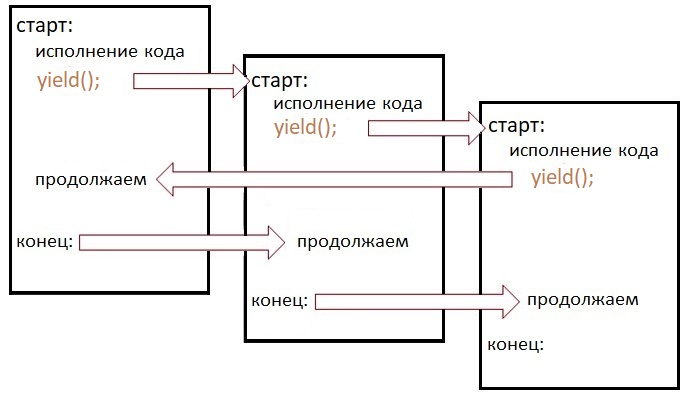
\includegraphics[scale=0.5]{images/scheme.jpg}
	\par
	Подходы к реализации:
	\begin{itemize}
		\item OpenJDK: копирование стека сопрограммы при переключении.
		\item HuaweiJDK : изменение указателя стека.
	\end{itemize}
\end{frame}

\begin{frame}{Сборка мусора}
	Что-то про сборку мусора
\end{frame}	
	
\begin{frame}{Результаты}
	\begin{itemize}
	\item Создан набор тестов производительности для языков Kotlin, Go, Java("Loom Project").
	\item Реализовано переключение контекста сопрограмм.
	\item Реализована трассировка ссылок объектов на стеках сопрограмм(???).
	\item Получены результаты тестов производительности.
	\end{itemize}
\end{frame}

\begin{frame}{Результаты: скорости переключения}
	Ubuntu, x64, 31 Гб ОЗУ
	\par Каждое значение усреднено по 100 измерениям.
	\begin{table}[H]
		%\caption{Число переключений корутин}\label{inc-matrix}
		\begin{tabular}{|c|c|c|c|c|c|}
			\hline \multirow{2}{*}{Cопрограмм, шт.} & \multicolumn{2}{|c|}{Число переключений, 1/сек.}    \\
			\cline{2-3}    & HuaweiJDK          & OpenJDK                \\% & Go                        \\
			\hline 100     & 483'656 (-/+ 4'113) & 1'900'009 (-/+ 19'732)\\% & 18'187'799 (-/+ 219367)   \\
			\hline 1000    & 476'467 (-/+ 4'517) & 1'775'239 (-/+ 20'491)\\% & 17'934'078 (-/+ 332778)   \\
			\hline 5000    & 435'239 (-/+ 2'942) & 1'703'631 (-/+ 30'498)\\% & 12'892'417 (-/+ 339410)   \\ % 
			\hline 10000   & 419'376 (-/+ 4'266) & 1'924'971 (-/+ 234982)\\% & 8'307'791 (-/+ 79652)     \\ % 
			\hline 50000   & 372'378 (-/+ 2'719) & 1'518'349 (-/+ 152899)\\% & 5'292'780 (-/+ 121844)    \\ % 
			\hline 
		\end{tabular}
	\end{table}
	
\end{frame}

\begin{frame}{Результаты: потребление памяти}
	Ubuntu, x64, 31 Гб ОЗУ
	\begin{table}[H]
		%\caption{Число переключений корутин}\label{inc-matrix}
		\begin{tabular}{|c|c|c|c|c|c|}
			\hline \multirow{2}{*}{Число сопрограмм, шт.} & \multicolumn{3}{|c|}{Размер физической памяти, 1/сек.}    \\
			\cline{2-4}    & HuaweiJDK & OpenJDK  & Go   \\
			\hline 100     & 34M       & 130M     & 3040K  \\
			\hline 1000    & 38M       & 161M     & 3105K  \\
			\hline 5000    & 59M       & 187M     & 3156K  \\
			\hline 10000   & 85M       & 193M     & 3308K \\
			\hline 50000   & 287M      & 202M     & 3407K  \\ 
			\hline 
		\end{tabular}
	\end{table}
\end{frame}


\begin{frame}{Применение сопрограмм.}
	\begin{itemize}
	\item Реализация бесконечных списков, итераторов, генераторов.
	\item Написание асинхронного и неблокирующего кода (та причина, из-за которой сопрограммы стали востребованы сейчас)
	\end{itemize}
\end{frame}

\begin{frame}{План дальнейших работ} 
	\begin{itemize}
	\item Переделать функцию переключения контекста.
	\item Реализация возможности миграции сопрограмм с одного потока на другой.
	\item Синхронизация: поддержка synchronized блоков.
	\item Переключение сопрограммы при вызове ввода вывода.
	\end{itemize}
\end{frame}

\begin{frame}
	\begin{center}
		Спасибо за внимание!
	\end{center}
\end{frame}

